\documentclass[a4paper,16pt]{article}
\usepackage[T2A]{fontenc}
\usepackage{amsmath,amsfonts,amssymb}
\usepackage{mathtools}
\usepackage{cancel}  % зачёркивание
\usepackage[dvipsnames]{xcolor}
\usepackage[english]{babel}
\usepackage{graphicx} % Required for inserting images
\graphicspath{ {./images/} }

\def\mathunderline#1#2{\color{#1}\underline{{\color{black}#2}}\color{black}}
\newcommand\Ccancel[2][black]{\renewcommand\CancelColor{\color{#1}}\cancel{#2}}

\title{\textbf{Пояснения к двойному маятнику}}
\date{}

\begin{document}
\maketitle

\begin{figure}[h]
    \centering
    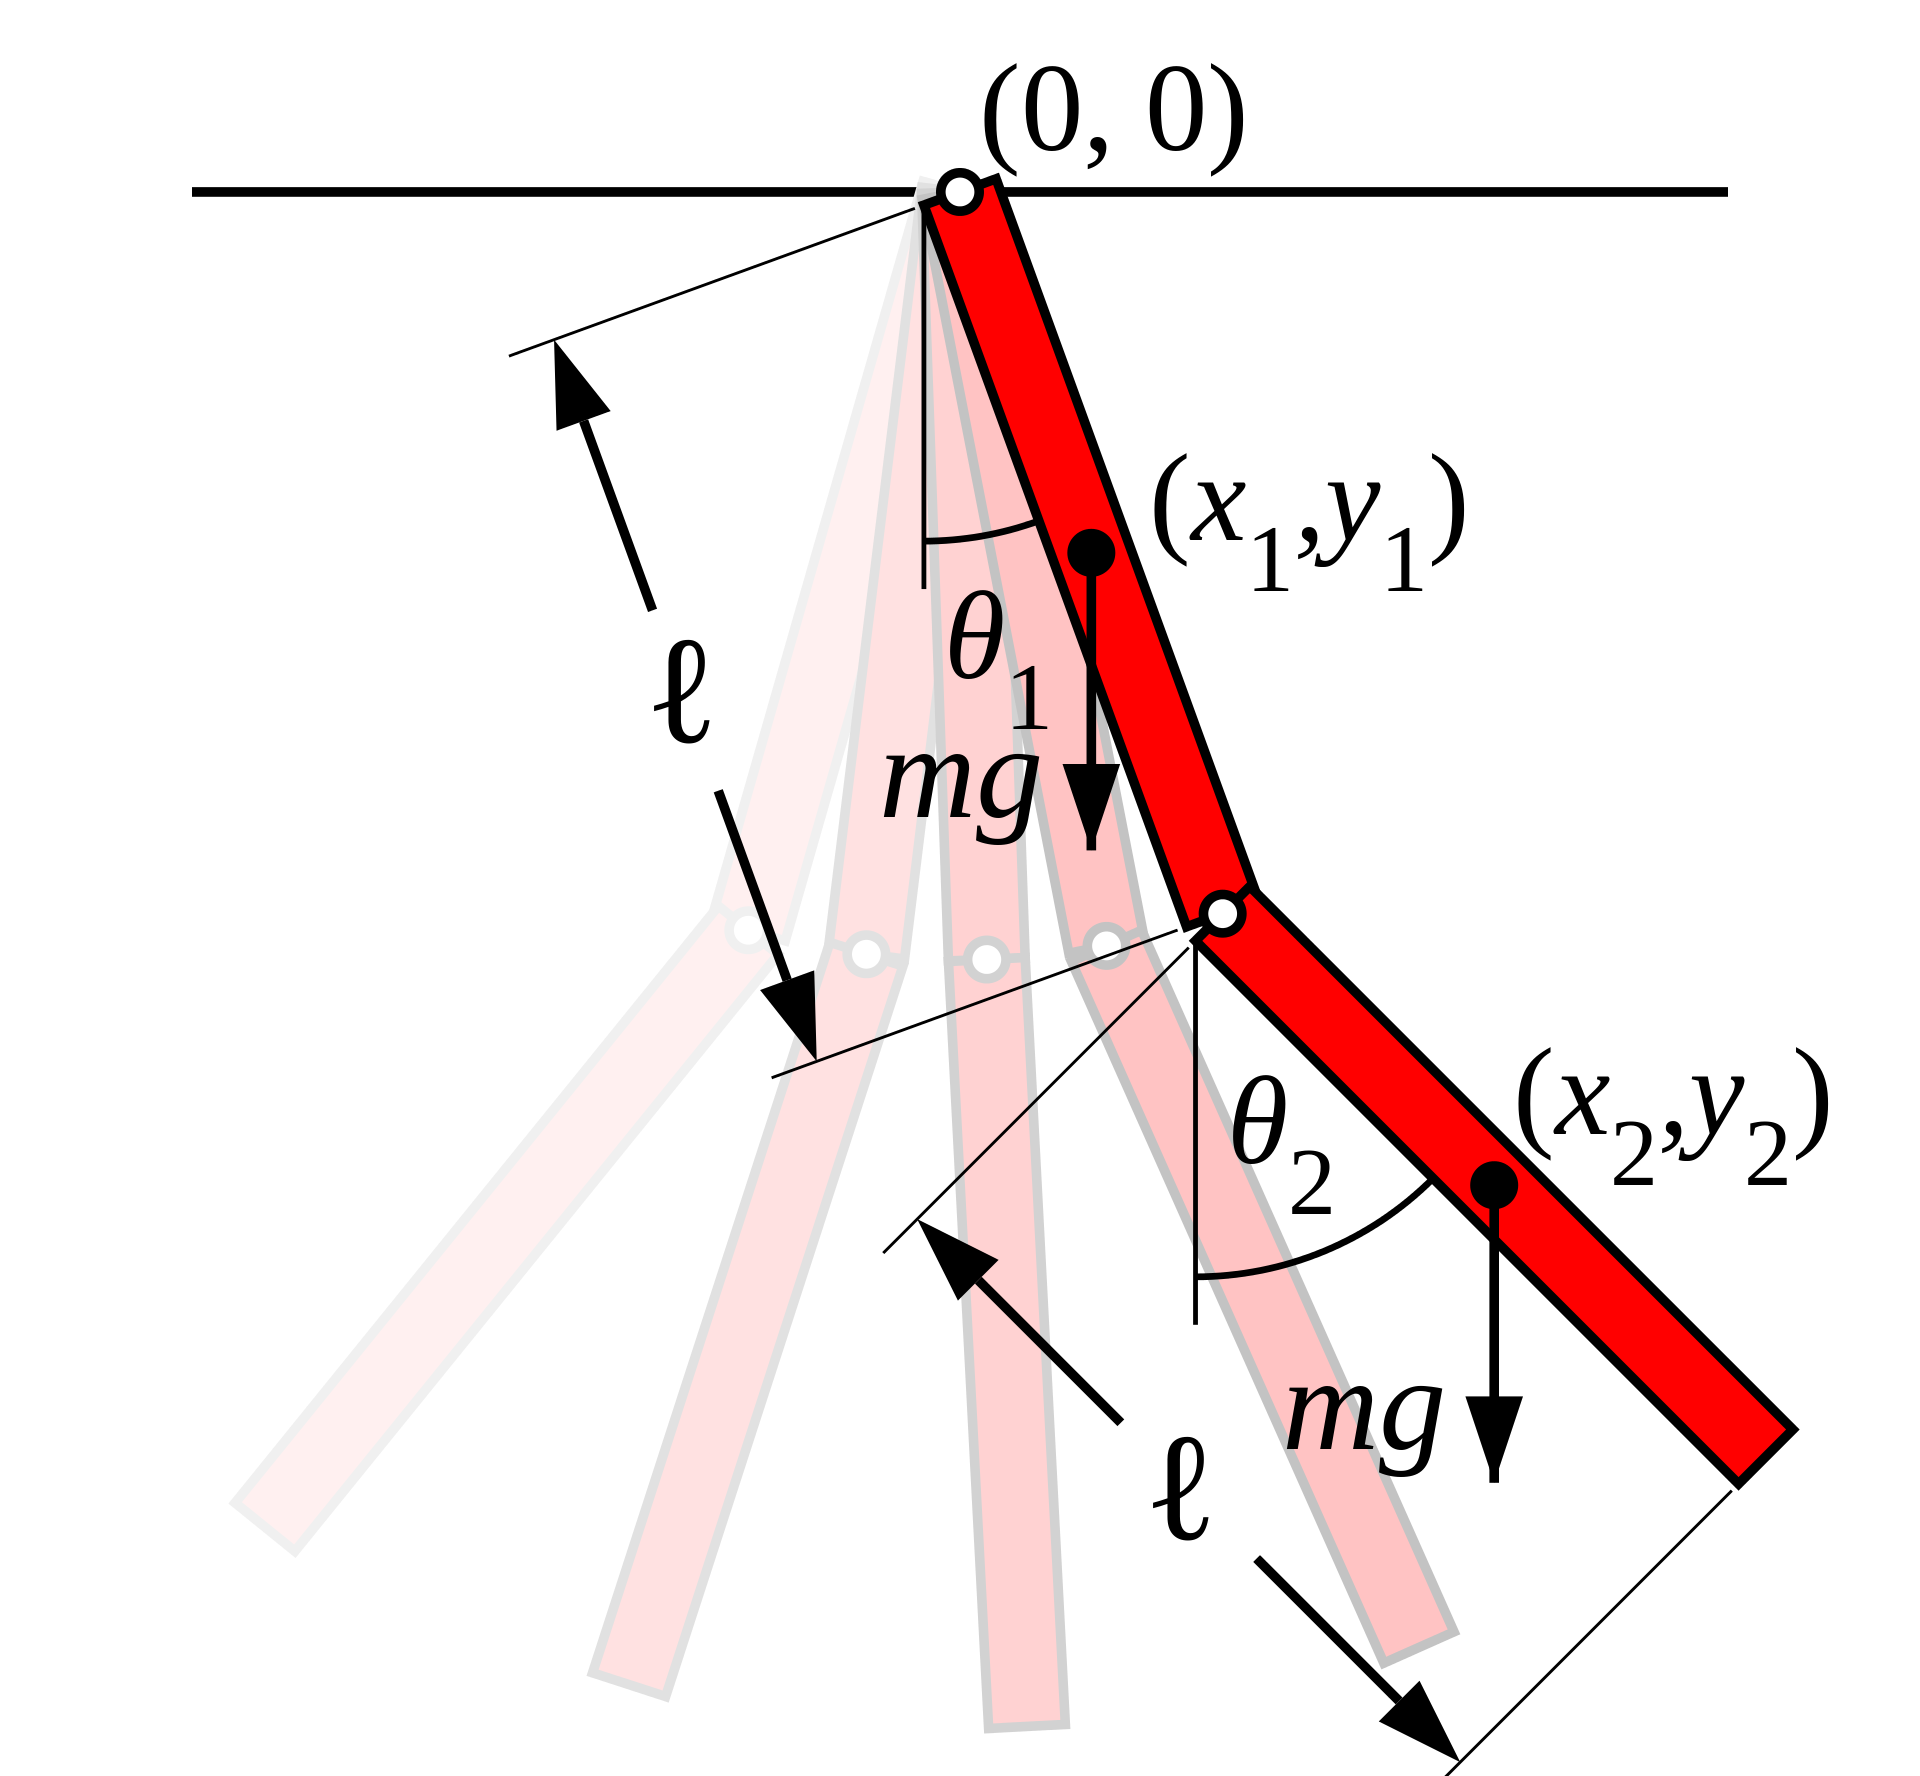
\includegraphics[width=0.5\linewidth]{pend.png}
\end{figure}

Рассмотрим случай, когда длины и массы маятников одинаковы ($m \text{ и } l$).
Тогда координаты центра масс первого звена $(x_1,y_1)$ - это
\begin{equation}
\begin{split}
&\begin{cases}
    x_1 = \frac{\ell}{2} \sin \theta_1 \\
    y_1 = -\frac{\ell}{2} \cos \theta_1
    \end{cases}
    \\ 
    &\begin{cases}
        x_2 = \ell \left (  \sin \theta_1 + \frac{1}{2} \sin \theta_2 \right )\\
        y_2 = -\ell \left (  \cos \theta_1 + \frac{1}{2} \cos \theta_2 \right ),
        \end{cases}
\end{split}
    \label{eq:1}
\end{equation}
а координаты центра масс второго звена - это конец первого
звена + проекции на x и y, с учётом угла $\theta_2$

Лагранжиан $L$ (в данном случае) - это разница \textcolor{red}{кинетической} энергии и \textcolor{blue}{потенциальной}.
При этом кинетическая энергия составляется из \textcolor{orange}{поступательной} и \textcolor{magenta}{вращательной}.
А момент инерции $I=\frac{1}{12} m \ell^2$
\begin{align}
    L & = \mathunderline{orange}{\frac{1}{2} m \left ( v_1^2 + v_2^2 \right )} + \mathunderline{pink}{\frac{1}{2} I \left ( {\dot \theta_1}^2 + {\dot \theta_2}^2 \right )} - \mathunderline{blue}{m g \left ( y_1 + y_2 \right )} \notag \\ 
    & = \frac{1}{2} m \left ( {\dot x_1}^2 + {\dot y_1}^2 + {\dot x_2}^2 + {\dot y_2}^2 \right ) + \frac{1}{2} I \left ( {\dot \theta_1}^2 + {\dot \theta_2}^2 \right ) - m g \left ( y_1 + y_2 \right )
\end{align} 

Подставив в (2) $x_1, \; y_1, \; x_2, \;y_2$ из (1), получим
\begin{equation}
    L = \frac{1}{6} m \ell^2 \left [ {\dot \theta_2}^2 +
    4 {\dot \theta_1}^2 + 3 {\dot \theta_1} {\dot \theta_2} \cos (\theta_1-\theta_2) \right ]
    + \frac{1}{2} m g \ell \left ( 3 \cos \theta_1 + \cos \theta_2 \right )
    \label{eq:3}
\end{equation}
Для того, чтобы найти уравнения движения двойного маятника, продифференцируем
Лагранжиан $L$ по $\dot{\theta_1}$ и $\dot{\theta_2}$.

Тогда
\[
    \begin{split}
   & \frac{\partial L}{\partial {\dot \theta_1} } = 
    \frac{\partial }{\partial {\dot \theta_1} } \left[ 
     \frac{1}{6} m \ell^2 \left [ \Ccancel[red]{ {\dot \theta_2}^2} +
    4 {\dot \theta_1}^2 + 3 {\dot \theta_1} {\dot \theta_2} \cos (\theta_1-\theta_2) \right ]
    + \Ccancel[red]{ \frac{1}{2} m g \ell \left ( 3 \cos \theta_1 + \cos \theta_2 \right )} \right] \\
    %
   & \frac{\partial L}{\partial {\dot \theta_2} } =
    \frac{\partial }{\partial {\dot \theta_2} } \left[ 
     \frac{1}{6} m \ell^2 \left [ {\dot \theta_2}^2 +
    \Ccancel[red]{4 {\dot \theta_1}^2} + 3 {\dot \theta_1} {\dot \theta_2} \cos (\theta_1-\theta_2) \right ]
    +  \Ccancel[red]{\frac{1}{2} m g \ell \left ( 3 \cos \theta_1 + \cos \theta_2 \right )} \right]
    \end{split}
\]
\[
    \begin{cases}
        p_{\theta_1} \equiv \frac{\partial L}{\partial {\dot \theta_1}} = \frac{1}{6} m \ell^2 \left [ 8 {\dot \theta_1}  + 3 {\dot \theta_2} \cos (\theta_1-\theta_2) \right ]\\ \\
        p_{\theta_2} \equiv \frac{\partial L}{\partial {\dot \theta_2}} = \frac{1}{6} m \ell^2 \left [ 2 {\dot \theta_2} + 3 {\dot \theta_1} \cos (\theta_1-\theta_2)  \right ].
        \end{cases}
\]

Опустив дальнейшие шаги, получим систему из 4х уравнений:
\begin{equation}
    \begin{cases}
        {\dot \theta_1} = \dfrac{6}{m\ell^2} \dfrac{ 2 p_{\theta_1} - 3 \cos(\theta_1-\theta_2) p_{\theta_2}}{16 - 9 \cos^2(\theta_1-\theta_2)}\\ \\
        {\dot \theta_2} = \dfrac{6}{m\ell^2} \dfrac{ 8 p_{\theta_2} - 3 \cos(\theta_1-\theta_2) p_{\theta_1}}{16 - 9 \cos^2(\theta_1-\theta_2)} \\
        {\dot p_{\theta_1}} = -\frac{1}{2} m \ell^2 \left [ {\dot \theta_1} {\dot \theta_2} \sin (\theta_1-\theta_2) + 3 \frac{g}{\ell} \sin \theta_1 \right ]\\ \\
{\dot p_{\theta_2}} = -\frac{1}{2} m \ell^2 \left [ -{\dot \theta_1} {\dot \theta_2} \sin (\theta_1-\theta_2) +  \frac{g}{\ell} \sin \theta_2 \right ].
\end{cases}
    \label{eq: фин_система}
\end{equation}

Тогда, с помощью численного интегрирования д.у., можно найти значения
углов отклонения маятника.
Обратите внимание, что (\ref{eq: фин_система}) - это система из 4-х дифференциальных
уравнений первого порядка. И можно применить метод Рунге-Кутты (4-го порядка, например).
\end{document}